\begingroup
\definecolor{stepfill}{HTML}{F8FAFC}
\definecolor{stepborder}{HTML}{475569}
\definecolor{arrowcol}{HTML}{64748B}
\definecolor{steptext}{HTML}{1E293B}

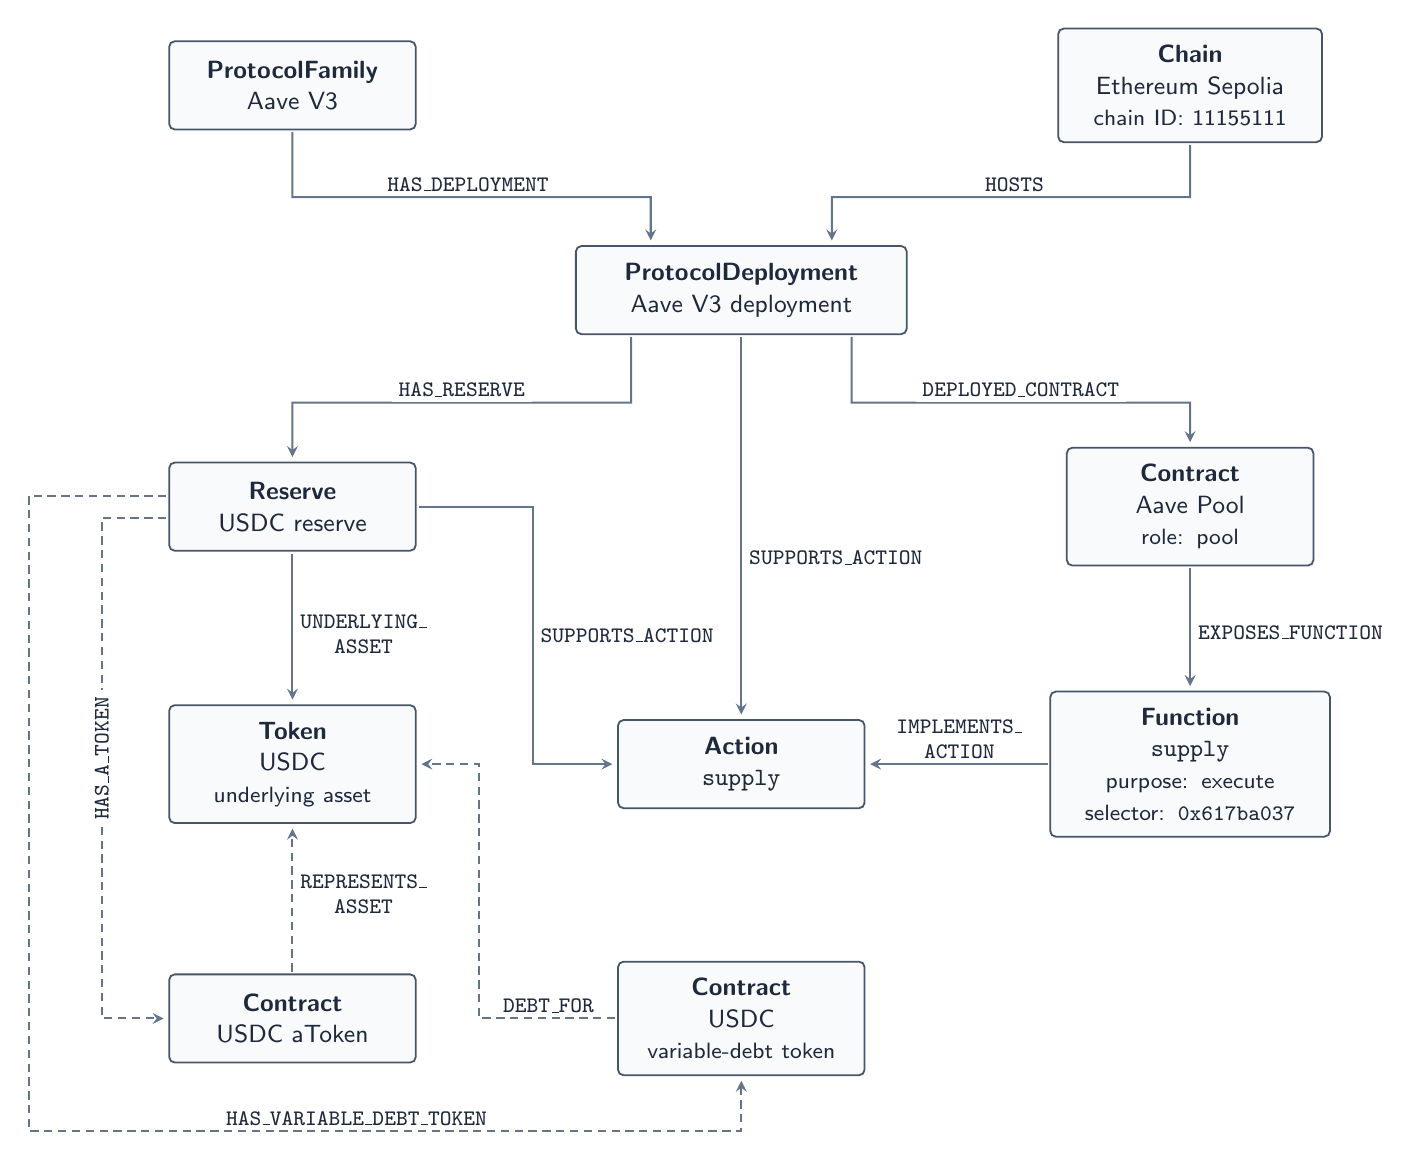
\begin{tikzpicture}[
  >=stealth,
  graphnode/.style={
    draw=stepborder,
    fill=stepfill,
    text=steptext,
    rounded corners=2pt,
    line width=0.65pt,
    text width=2.78cm,
    minimum height=1.12cm,
    inner xsep=5pt,
    inner ysep=6pt,
    outer sep=0pt,
    align=center,
    font=\sffamily\fontsize{9.4}{11.4}\selectfont
  },
  edge/.style={
    ->,
    draw=arrowcol,
    line width=0.74pt,
    shorten <=1pt,
    shorten >=2pt
  },
  contextedge/.style={
    edge,
    densely dashed
  },
  rel/.style={
    fill=white,
    text=steptext,
    align=center,
    inner xsep=2.5pt,
    inner ysep=1.7pt,
    font=\ttfamily\fontsize{7.7}{9.0}\selectfont
  }
]

% --------------------------------------------------
% Nodes
% --------------------------------------------------

\node[graphnode] (family) at (-5.70,0)
  {\textbf{ProtocolFamily}\\Aave V3};

\node[graphnode,text width=3.00cm] (chain) at (5.70,0)
  {\textbf{Chain}\\Ethereum Sepolia\\
   {\footnotesize chain ID: 11155111}};

\node[graphnode,text width=3.85cm] (deployment)
  at (0,-2.60)
  {\textbf{ProtocolDeployment}\\Aave V3 deployment};

\node[graphnode] (reserve) at (-5.70,-5.35)
  {\textbf{Reserve}\\USDC reserve};

\node[graphnode] (pool) at (5.70,-5.35)
  {\textbf{Contract}\\Aave Pool\\
   {\footnotesize role: pool}};

\node[graphnode] (token) at (-5.70,-8.62)
  {\textbf{Token}\\USDC\\
   {\footnotesize underlying asset}};

\node[graphnode] (action) at (0,-8.62)
  {\textbf{Action}\\\texttt{supply}};

\node[graphnode,text width=3.20cm] (fn)
  at (5.70,-8.62)
  {\textbf{Function}\\\texttt{supply}\\
   {\footnotesize purpose: execute}\\
   {\footnotesize selector: \texttt{0x617ba037}}};

\node[graphnode] (atoken) at (-5.70,-11.85)
  {\textbf{Contract}\\USDC aToken};

\node[graphnode] (debt) at (0,-11.85)
  {\textbf{Contract}\\USDC\\
   {\footnotesize variable-debt token}};

% --------------------------------------------------
% Protocol and chain relationships
% --------------------------------------------------

\draw[edge]
  (family.south) -- (-5.70,-1.42)
  -- node[rel,above,pos=0.49]
     {HAS\_DEPLOYMENT} (-1.15,-1.42)
  -- ([xshift=-1.15cm]deployment.north);

\draw[edge]
  (chain.south) -- (5.70,-1.42)
  -- node[rel,above,pos=0.49]
     {HOSTS} (1.15,-1.42)
  -- ([xshift=1.15cm]deployment.north);

% --------------------------------------------------
% Deployment relationships
% --------------------------------------------------

\draw[edge]
  ([xshift=-1.40cm]deployment.south)
  -- (-1.40,-4.03)
  -- node[rel,above,pos=0.50]
     {HAS\_RESERVE} (-5.70,-4.03)
  -- (reserve.north);

\draw[edge]
  ([xshift=1.40cm]deployment.south)
  -- (1.40,-4.03)
  -- node[rel,above,pos=0.50]
     {DEPLOYED\_CONTRACT} (5.70,-4.03)
  -- (pool.north);

\draw[edge]
  (deployment.south)
  -- node[rel,right,pos=0.58]
     {SUPPORTS\_ACTION}
  (action.north);

% --------------------------------------------------
% Reserve and action relationships
% --------------------------------------------------

\draw[edge]
  (reserve.south)
  -- node[rel,right,pos=0.54]
     {UNDERLYING\_\\ASSET}
  (token.north);

\draw[edge]
  (reserve.east)
  -- (-2.65,-5.35)
  -- node[rel,right,pos=0.50]
     {SUPPORTS\_ACTION} (-2.65,-8.62)
  -- (action.west);

% --------------------------------------------------
% Contract and function relationships
% --------------------------------------------------

\draw[edge]
  (pool.south)
  -- node[rel,right,pos=0.53]
     {EXPOSES\_FUNCTION}
  (fn.north);

\draw[edge]
  (fn.west)
  -- node[rel,above,pos=0.49]
     {IMPLEMENTS\_\\ACTION}
  (action.east);

% --------------------------------------------------
% Supplementary reserve-token relationships
% Dashed edges distinguish contextual graph knowledge.
% --------------------------------------------------

% Reserve -> aToken
\draw[contextedge]
    ([yshift=-4pt]reserve.west)
    -| (-8.12,-11.85)
    -- (atoken.west);

\node[rel, rotate=90]
    at (-8.12,-8.55)
    {HAS\_A\_TOKEN};

% Reserve -> variable-debt token
\draw[contextedge]
    ([yshift=4pt]reserve.west)
    -| (-9.05,-13.28)
    -- node[rel,above,pos=0.46]
       {HAS\_VARIABLE\_DEBT\_TOKEN}
       (0,-13.28)
    -- (debt.south);

% aToken -> underlying asset
\draw[contextedge]
  (atoken.north)
  -- node[rel,right,pos=0.53]
     {REPRESENTS\_\\ASSET}
  (token.south);

% Variable-debt token -> underlying asset
\draw[contextedge]
  (debt.west)
  -- node[rel,above,pos=0.50]
     {DEBT\_FOR} (-3.33,-11.85)
  -- (-3.33,-8.62)
  -- (token.east);

\end{tikzpicture}
\endgroup
